\subsection{Temperature and Salinity Changes}
To get a better picture of the changes that occur during the time periods we compare differences in sea temperature and salinity at 250m depth between the models. We do not use the sea surface temperature and salinity here because of the restoring boundary conditions used on the top layer of the ocean. It is important to note that these restoring boundary conditions with the simplified forcings make a discussion on the thermohaline circulation to be of limited value. But we can get an idea of what general changes occur.

First, we compare the temperature difference in the 55Ma basin and the 35Ma basin. We thus compare the temperature profiles of the late Paleocene to the late Eocene (\cref{fig:5535cooling}). Here we see substantial differences between the two. One of the key features of the Eocene seems to be a large amount of cooling in the southern Atlantic along with a heating in the southern pacific. Resulting from the large Increase in size of the southern subtropical gyre in the Indian ocean. 

\begin{figure}[H]
	\begin{subfigure}{\linewidth}
			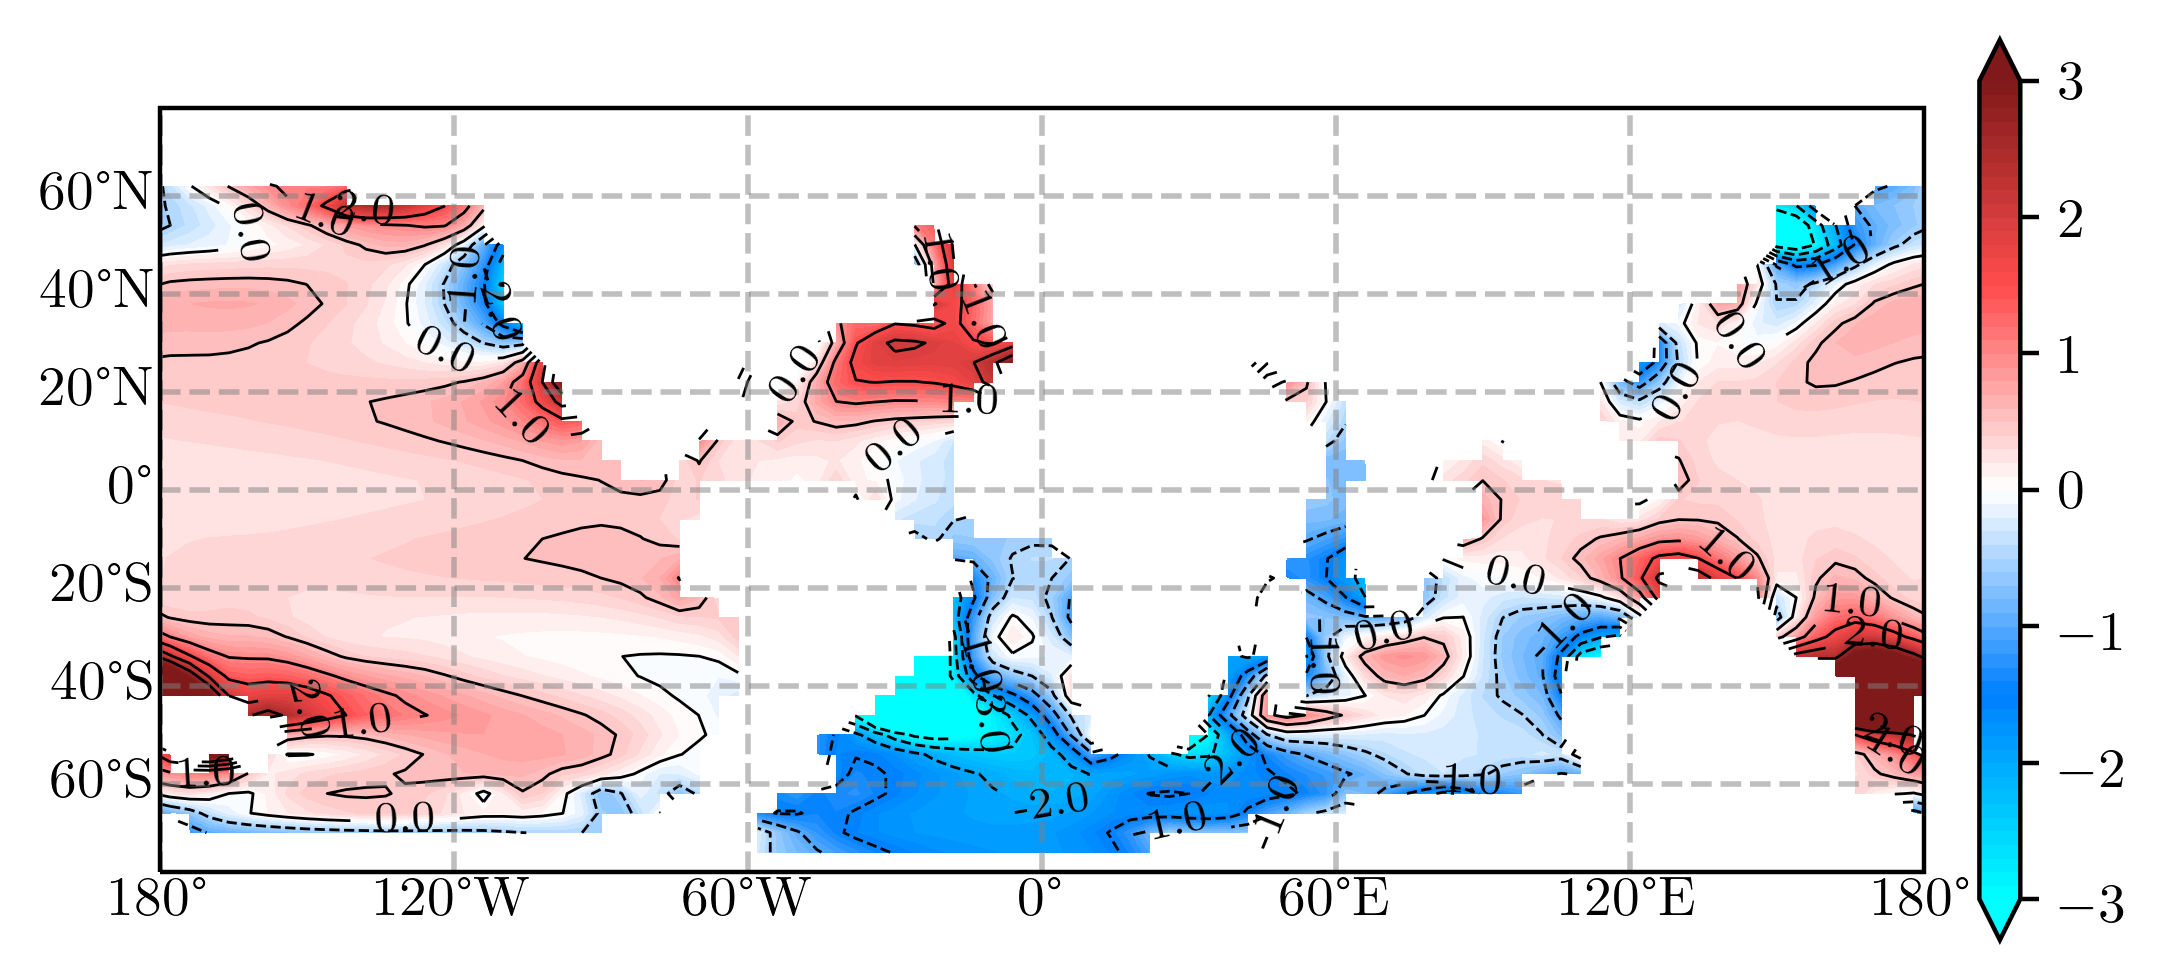
\includegraphics[width=\linewidth]{Paleo_eocene_55_35.png}
		\caption{Temperature $^{\circ}C$ diffirences between late Paleocene (55Ma) and late Eocene (35Ma) simulations. Positive values indicate warming, Negative values indicate cooling.}
		\label{fig:5535cooling}
	\end{subfigure}
	\begin{figure}{\linewidth}
		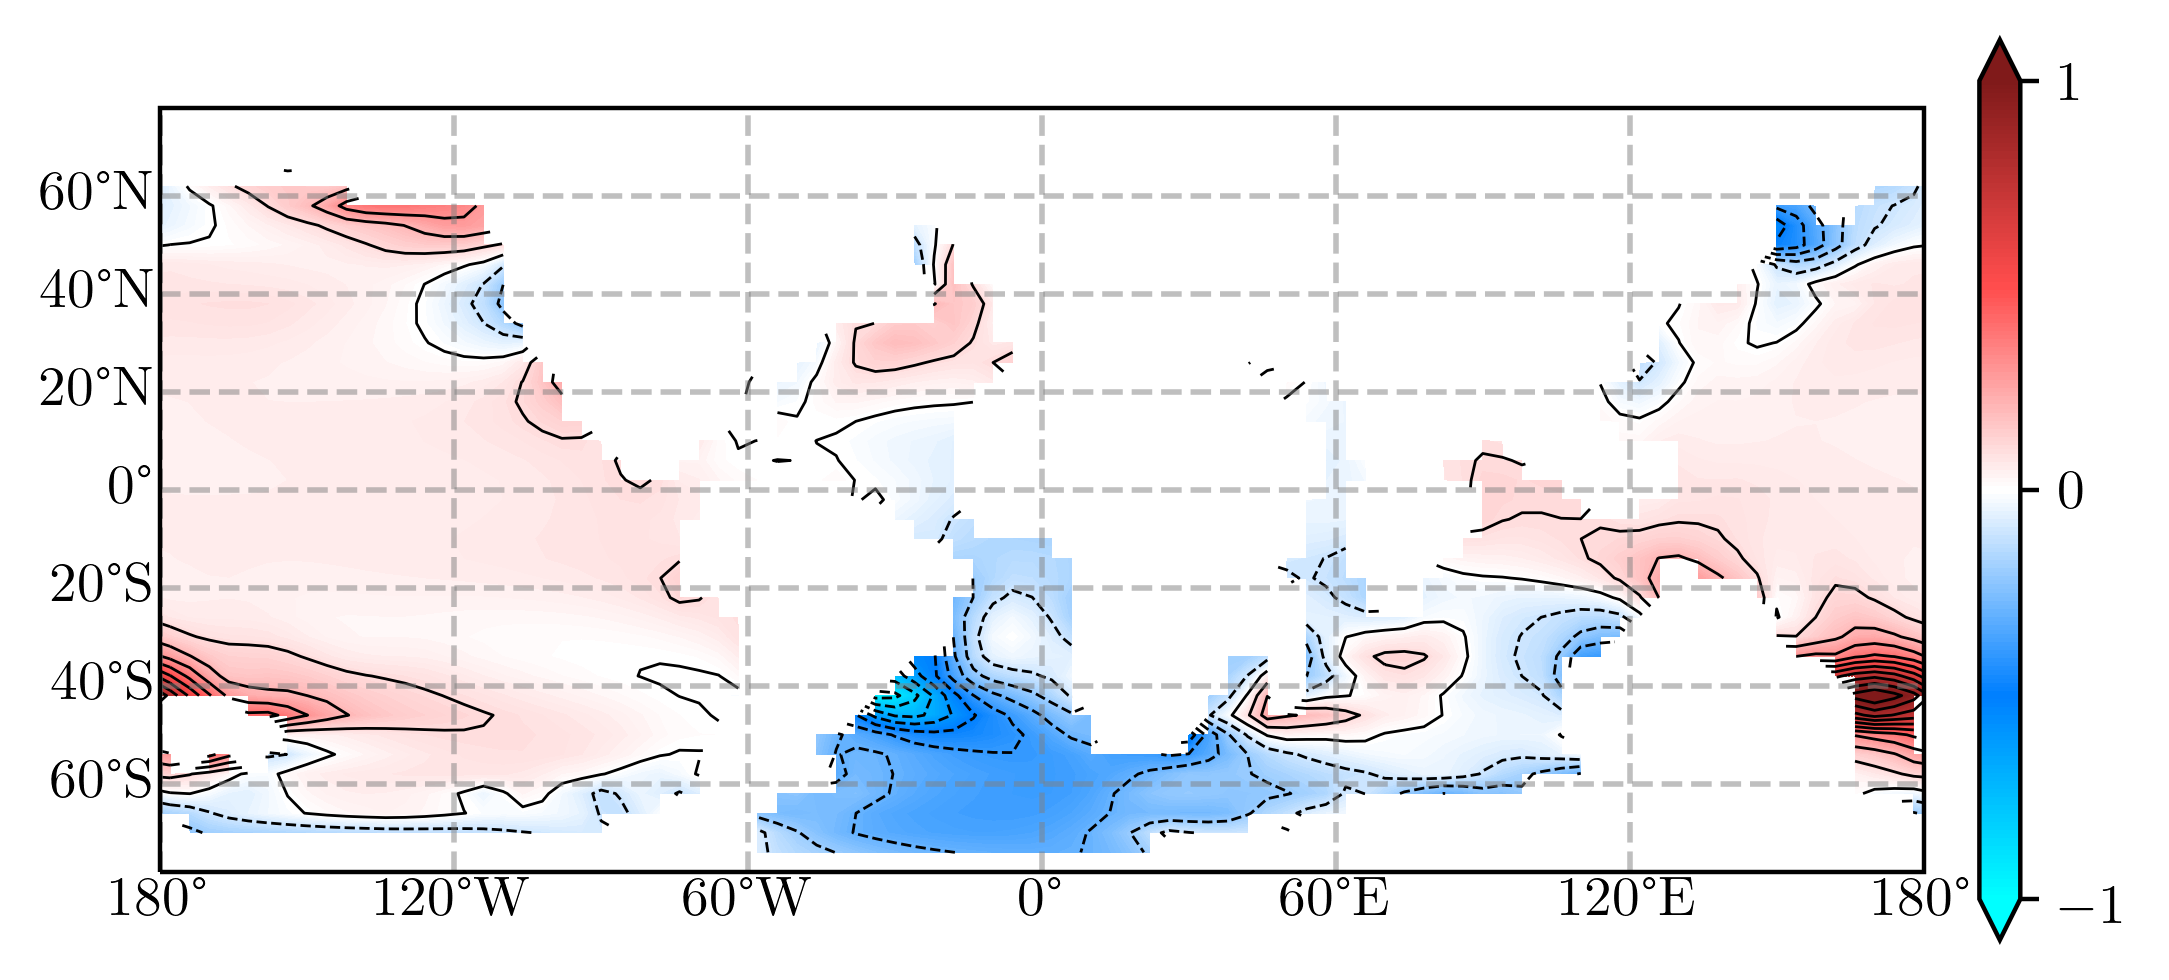
\includegraphics[width=\linewidth]{salt_55_35.png}
		\caption{Salinity (psu) diffirences between late Paleocene (55Ma) and late Eocene (35Ma) simulations at 245m depth. Positive values indicate warming, Negative values indicate cooling.}
		\label{fig:salt5535cooling}
	\end{figure}
	\caption{asdasd}
\end{figure}


We also look at the changes between the late Eocene and the late Oligocene. 

\begin{figure}[H]
	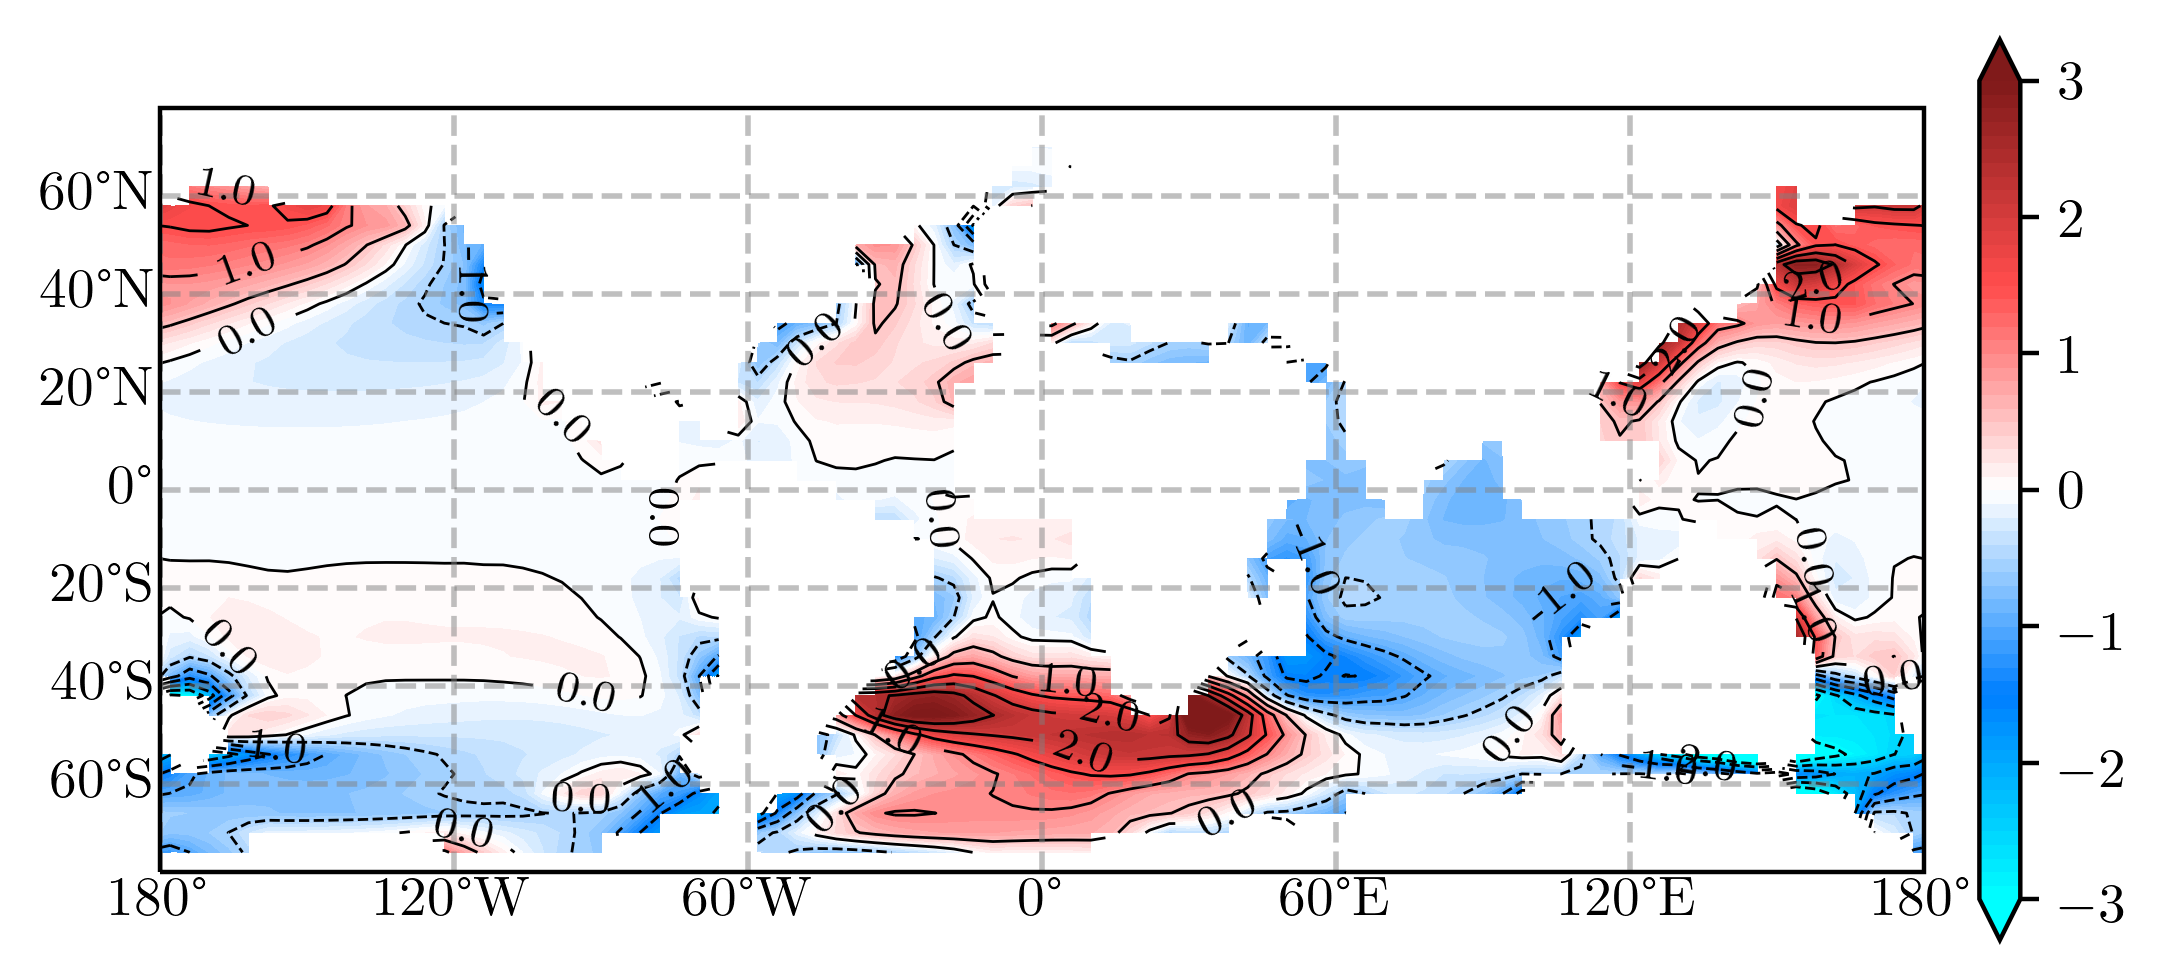
\includegraphics[width=\linewidth]{Paleo_eocene_35_20.png}
	\caption{Temperature $^{\circ}C$ diffirences between late Eocene (35Ma) and late Oligocene (20Ma) simulations. Positive values indicate warming, Negative values indicate cooling.}
	\label{fig:3520cooling}
\end{figure}

\begin{figure}[H]
	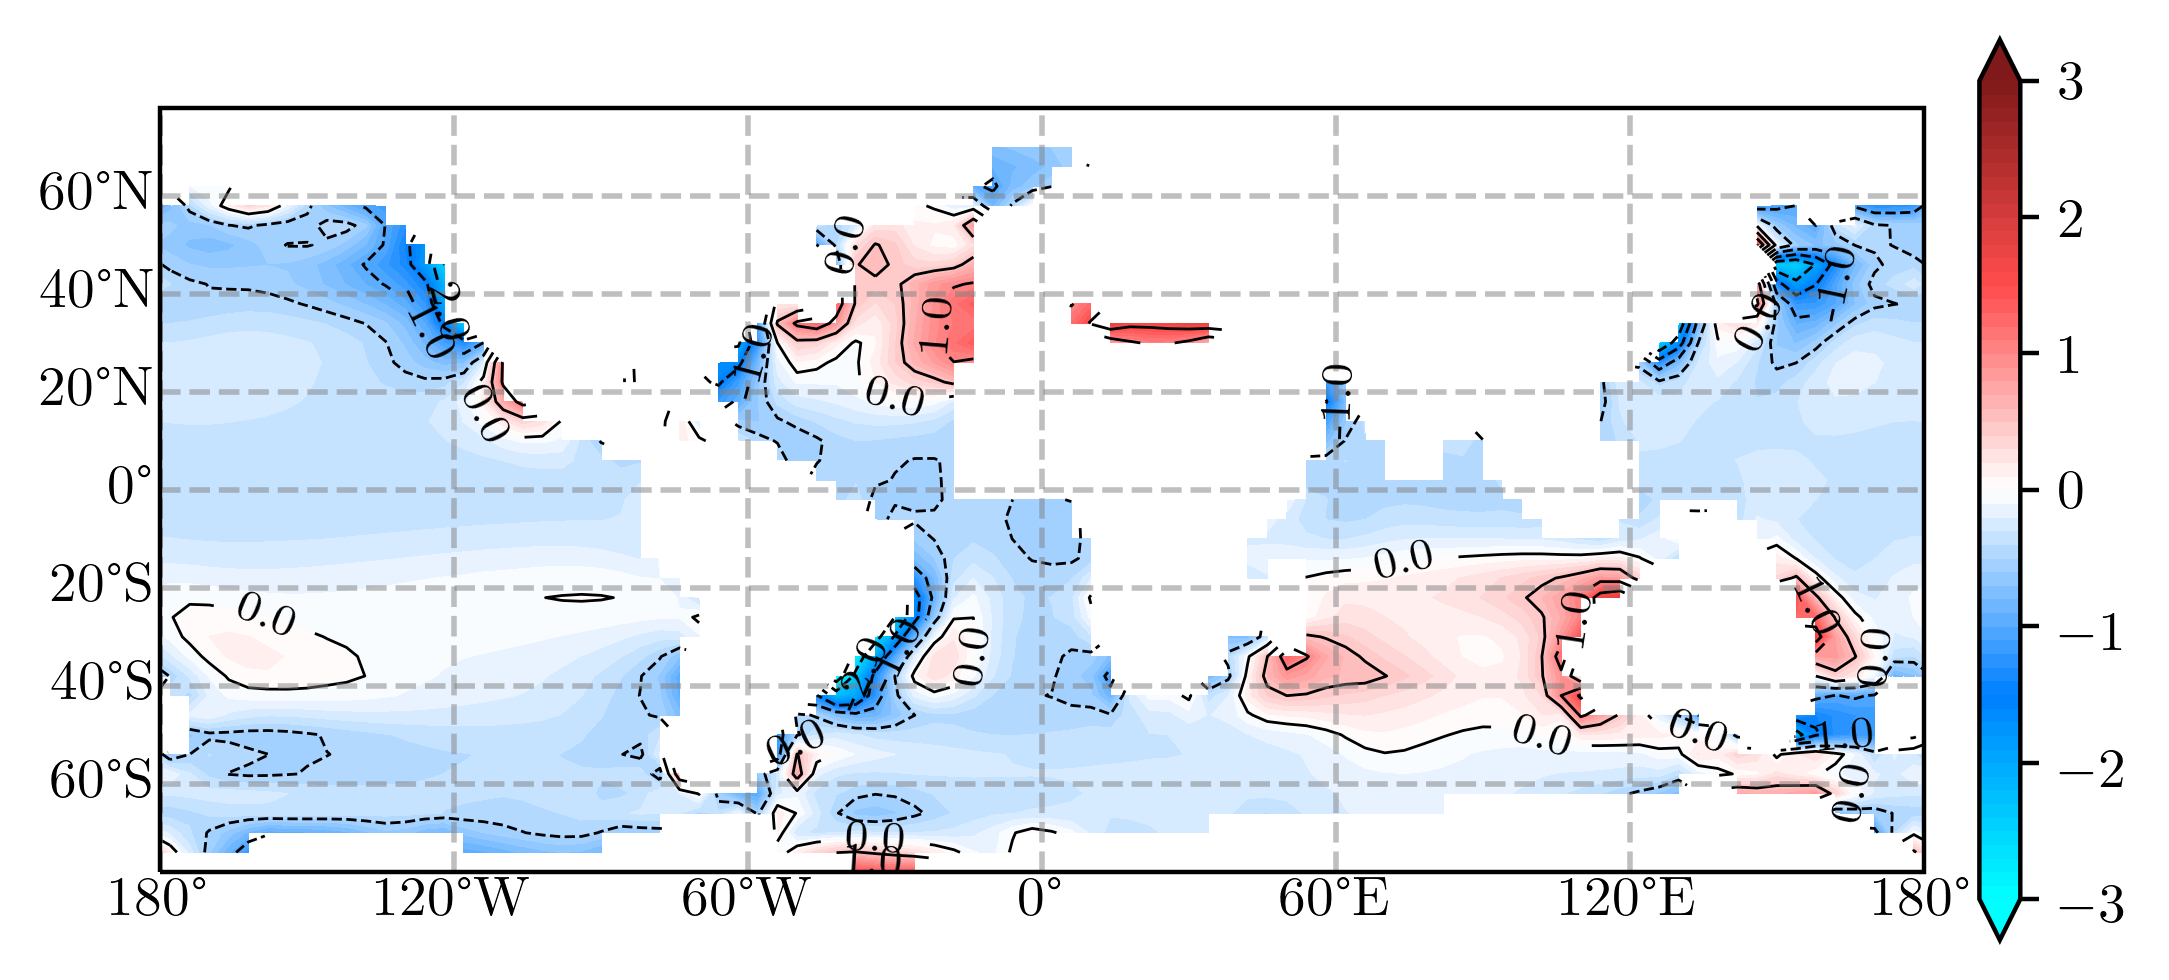
\includegraphics[width=\linewidth]{Paleo_eocene_20_10.png}
	\caption{Temperature diffirences $^{\circ}C$ between late Oligocene (20Ma) and middle Miocene (10Ma) simulations. Positive values indicate warming, Negative values indicate cooling.}
	\label{fig:2010cooling}
\end{figure}



\begin{figure}[H]
	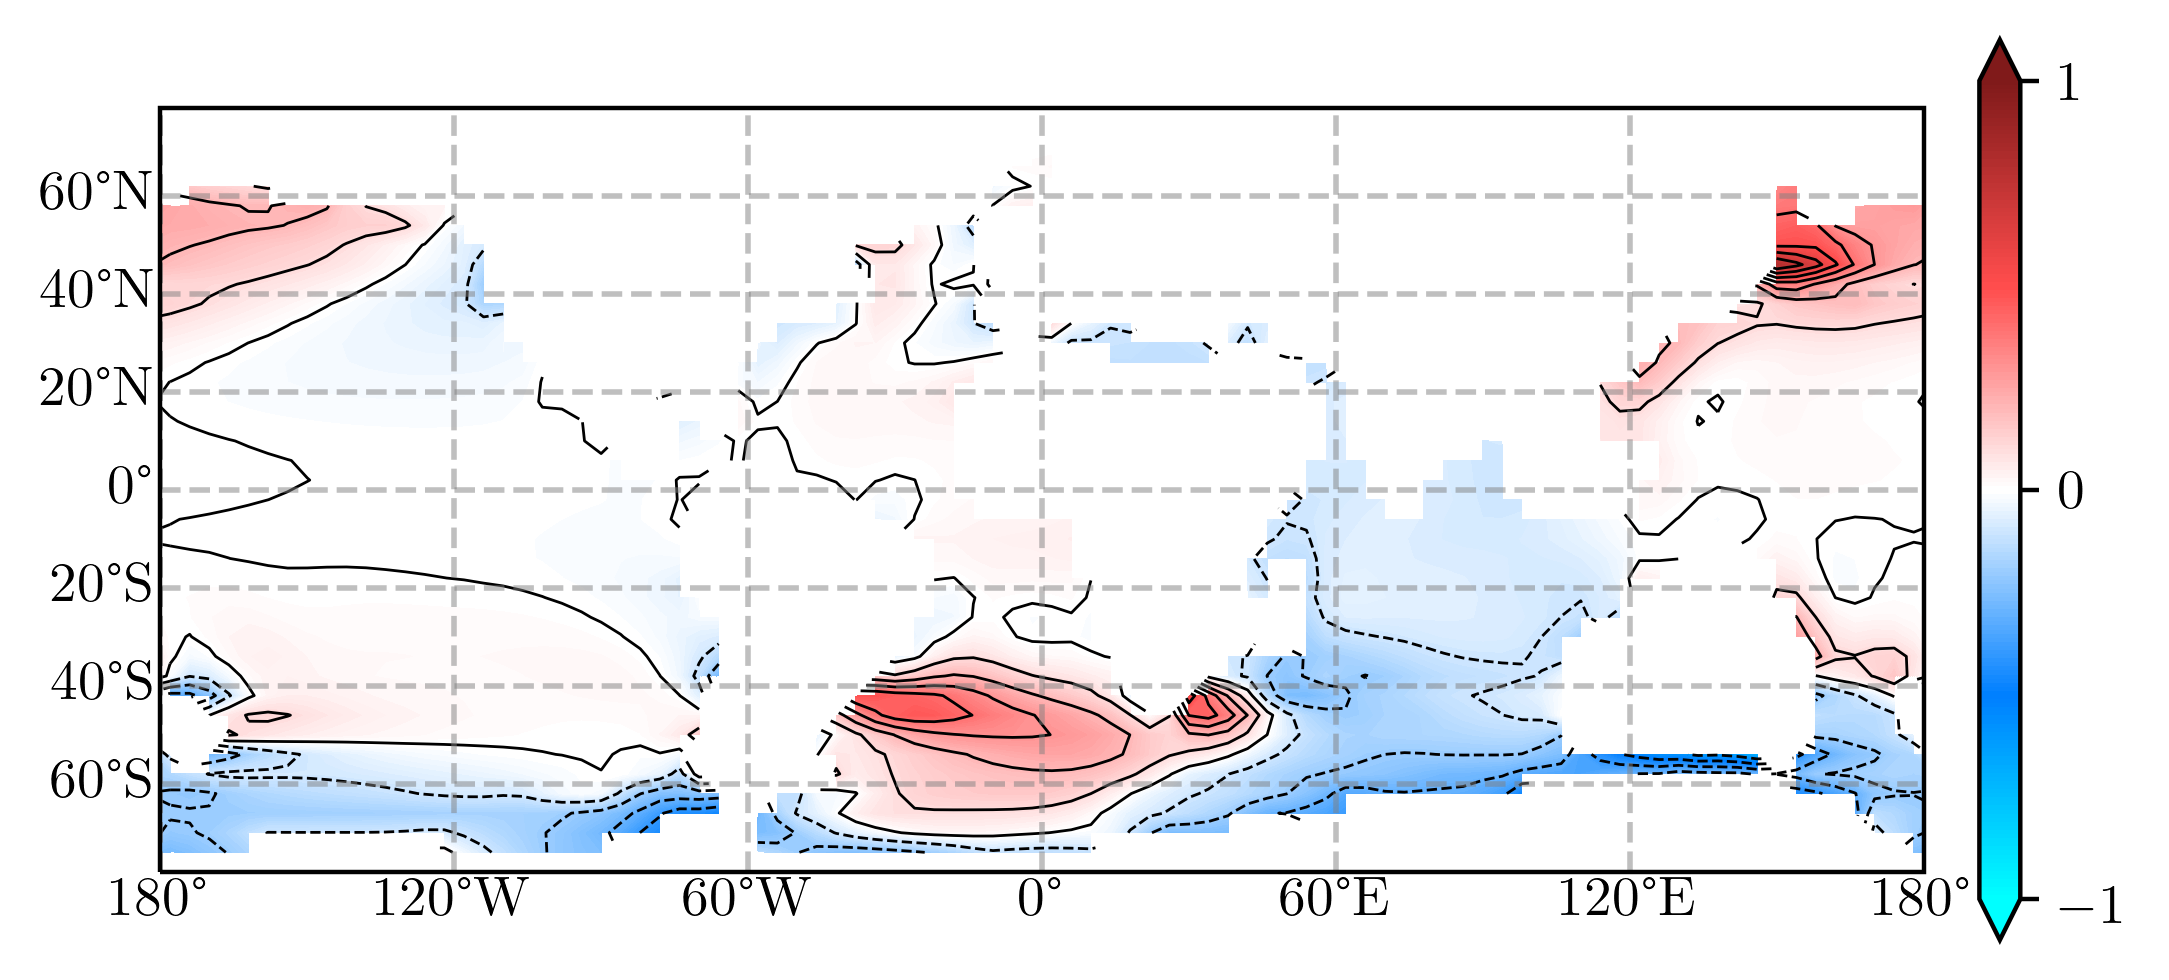
\includegraphics[width=\linewidth]{salt_35_20.png}
	\caption{Salinity (psu) diffirences between late Eocene (35Ma) and late Oligocene (20Ma) simulations at 245m depth. Positive values indicate warming, Negative values indicate cooling.}
	\label{fig:salt3520cooling}
\end{figure}
\begin{figure}[H]
	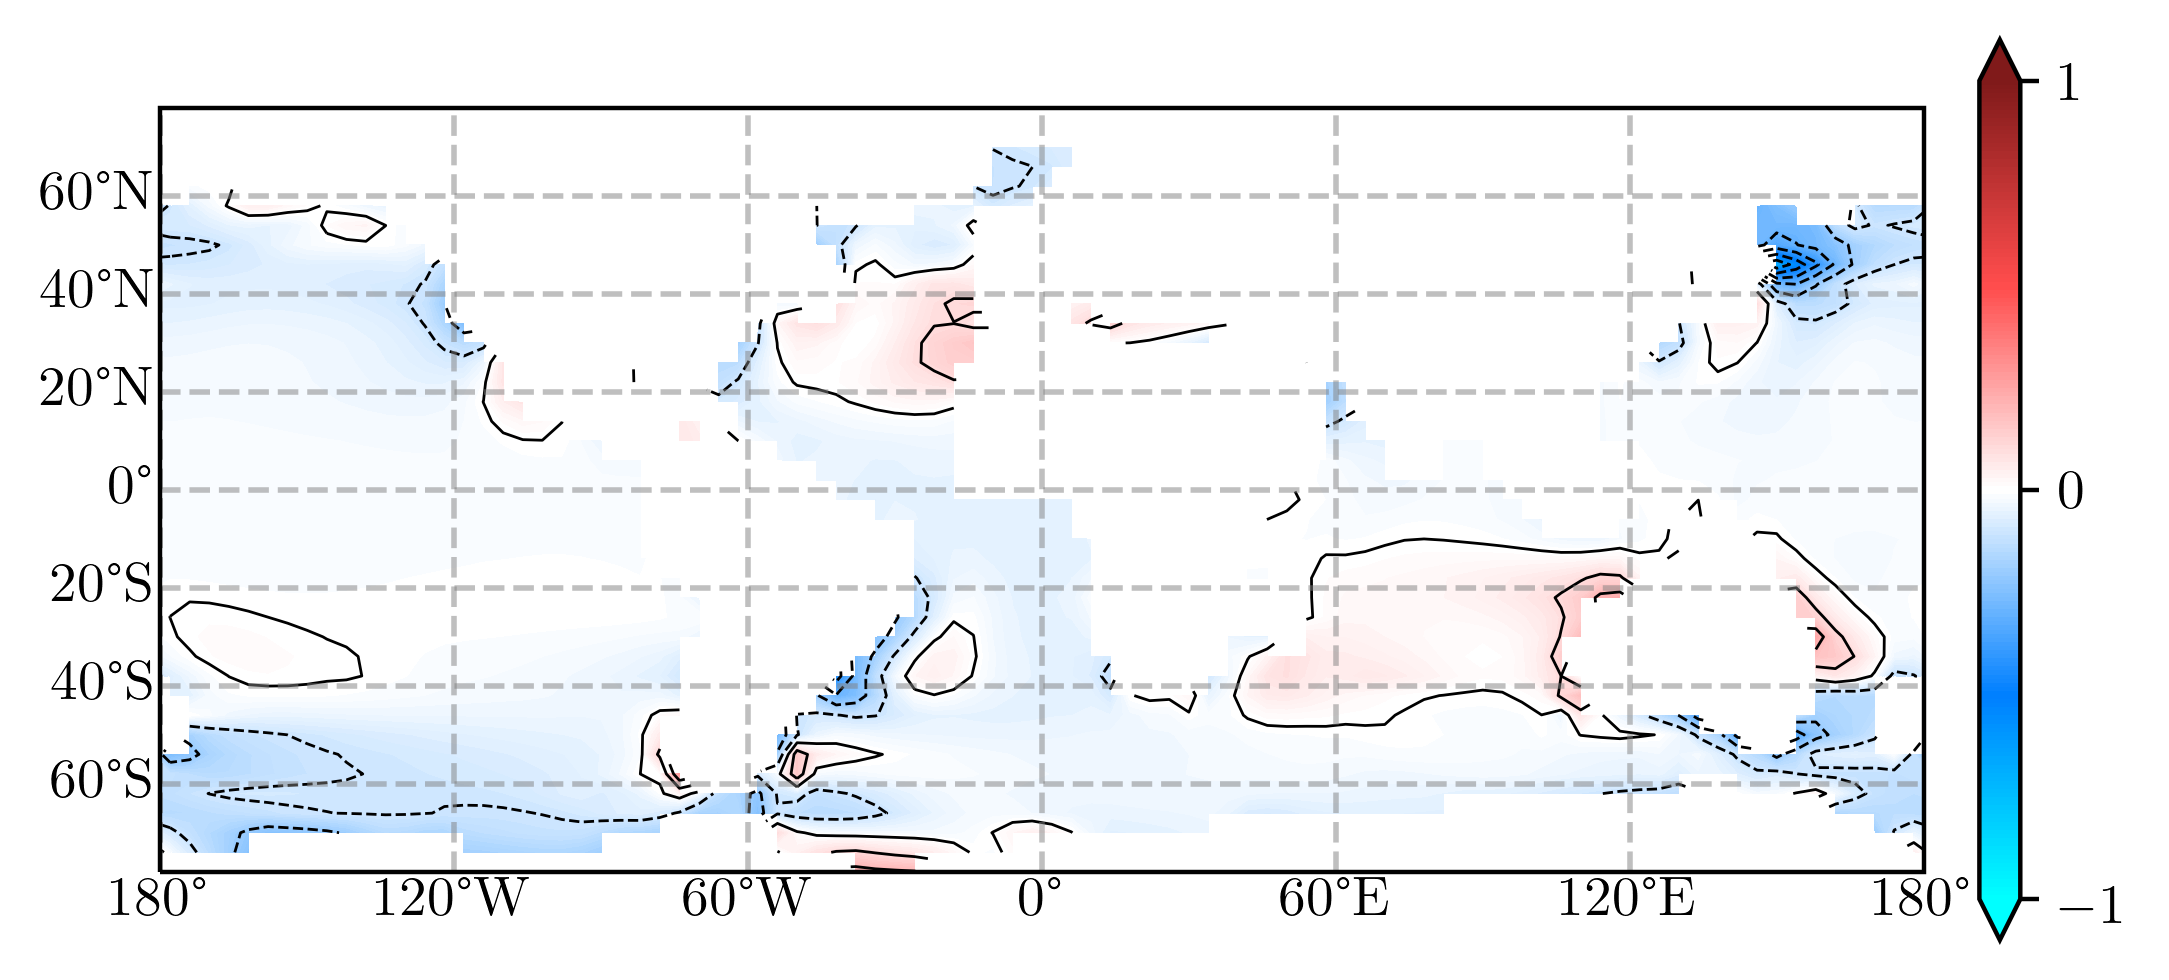
\includegraphics[width=\linewidth]{salt_20_10.png}
	\caption{Salinity (psu) diffirences between late Oligocene (20Ma) and middle Miocene (10Ma) simulations at 245m depth. Positive values indicate warming, Negative values indicate cooling.}
	\label{fig:salt2010cooling}
\end{figure}

